\documentclass[a4paper]{article}

\usepackage{tabularx}
\usepackage[portuguese]{babel}
\usepackage[utf8]{inputenc}
\usepackage{indentfirst}
\usepackage{graphicx}
\usepackage{verbatim}
\usepackage{wrapfig}
\usepackage{booktabs}
\usepackage{placeins}
\usepackage{listings}
\usepackage{color}
\usepackage{cite}
\usepackage{url}

\definecolor{dkgreen}{rgb}{0,0.5,0}
\definecolor{gray}{rgb}{0.5,0.5,0.5}
\definecolor{mauve}{rgb}{0.58,0,0.82}
\lstset{frame=tb,
  language=Prolog,
  aboveskip=3mm,
  belowskip=3mm,
  showstringspaces=false,
  columns=flexible,
  basicstyle={\small\ttfamily},
  numbers=none,
  numberstyle=\tiny\color{gray},
  keywordstyle=\color{blue},
  commentstyle=\color{dkgreen},
  stringstyle=\color{mauve},
  breaklines=true,
  breakatwhitespace=true,
  tabsize=3
}
\graphicspath{ {./img/} }

\begin{document}

\setlength{\textwidth}{16cm}
\setlength{\textheight}{22cm}

\title{\Huge\textbf{Adaptoid}\linebreak\linebreak\linebreak
\Large\textbf{Relatório Final}\linebreak\linebreak
\linebreak\linebreak

\includegraphics[scale=0.1]{feup-logo.png}\linebreak\linebreak
\linebreak\linebreak
\Large{Mestrado Integrado em Engenharia Informática e Computação} \linebreak\linebreak
\Large{Programação em Lógica}\linebreak
}

\author{\textbf{Grupo 04 : Adaptoid}\\ David Azevedo - 201405846 \\ João Ferreira - 201404332 \\\linebreak\linebreak \\
 \\ Faculdade de Engenharia da Universidade do Porto \\ Rua Roberto Frias, s\/n, 4200-465 Porto, Portugal \linebreak\linebreak\linebreak
\linebreak\linebreak\vspace{1cm}}
\date{Novembro de 2016}
\maketitle
\thispagestyle{empty}

%************************************************************************************************
%************************************************************************************************

\newpage

\section*{Resumo}
O problema abordado consitiu na implementação do jogo de tabuleiro "Adaptoid" na linguagem Prolog, o que nos representou como sendo um novo desafio, visto que, o grupo não estava familiarizado com este paradigma de programação em lógica. Os objectivos do projecto incluiram : permitir três modos de utilização (Humano/Humano, Humano/Computador, Computador/Computador), incluir dois níveis de jogo para o computador, interface adequada em modo de texto. O trabalho foi elaborado com base em 5 passos fundamentais implementados pela seguinte ordem :
\begin{enumerate}
    \item Representação do tabuleiro em Prolog usando códigos ASCII.
    \item Implementação das regras do jogo em predicados lógicos.
    \item Criação de uma interface simples com o utilizador.
    \item Desenvolvimento de uma pseudo AI para as jogadas do computador.
    \item Design de um sistema simples de menus para completar um ambiente de jogo.
\end{enumerate}

Todos os objectivos foram cumpridos sendo que temos um jogo completo e jogável desenvolvido em Prolog. Desenvolver um jogo funcional numa linguagem nova com a qual apenas se teve contacto durante algumas semana não é fácil, pelo que o grupo no inicio encontrou algumas dificuldades. Após uma leitura extensiva dos slides facultados pelos docentes assim como informação disponível na web foi possível obter uma melhor percepção desta linguagem e paradigma de programação por forma a desenvolver uma aplicação.


Concluindo, ambos os estudantes orgulham-se agora do resultado obtido e do método como tal foi alcançado, podemos também afirmar que o nosso conhecimento de Prolog aumentou consideravelmente.
\newpage

\tableofcontents

%************************************************************************************************
%************************************************************************************************

%*************************************************************************************************
%************************************************************************************************

\newpage

%%%%%%%%%%%%%%%%%%%%%%%%%%
\section{Introdução}

Este projecto foi proposto no âmbito da unidade curricular de Programação em Lógica do Mestrado Integrado de Engenharia Informática e de Computação. Consiste na adaptação de um jogo de tabuleiro para dois jogadores na linguagem Prolog. O tema escolhido foi o "Adaptoid" um jogo relativamente simples de compreender e aprender a jogar, mas que a quantidade de opções disponíveis ao jogador fazem com que o jogo tenha uma complexidade muito superior relativa ao que aparenta.
Este relatório tem a seguinte estrutura :
 \begin{itemize}
   \item Descrição do jogo, a sua história e regras.
   \item Implementação da lógica do jogo em Prolog.
   \item Forma de representação do estado do tabuleiro e sua visualização.
   \item Execução de movimentos.
   \item Verificação do cumprimento das regras do jogo.
   \item Determinação do final do jogo.
   \item Cálculo das jogadas a realizar pelo computador.
   \item Módulo de interface com o utilizador em modo de texto.
   \item Conclucões.
   \item Bibliografia.
   \item Anexos.
 \end{itemize}

\newpage
%%%%%%%%%%%%%%%%%%%%%%%%%%
\section{O Jogo Adaptoid}

\begin{wrapfigure}{r}{0.22\textwidth}
    \centering
    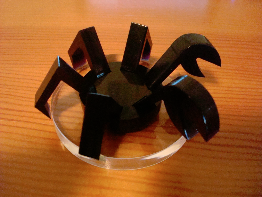
\includegraphics[width=0.22\textwidth]{adaptoid}
    \caption{Imagem ilustratica de um "adaptoid"}
\end{wrapfigure}

Adaptoid é um jogo de tabuleiro para dois jogadores, constituído por um tabuleiro hexagonal, que contém (37 espaços), e por um conjunto de criaturas denominadas de “adaptoid”. Cabe a cada jogador evoluir o seu “adaptoid” adicionando membros, garras e pernas, ao corpo do adaptoid. Os membros são fatores decisivos, pois fazem variar o comportamento do “adaptoid”. As garras definem o dano e as pernas a capacidade de movimento.

\begin{wrapfigure}{l}{0.20\textwidth}
    	\centering
	\vspace{-10pt}
   	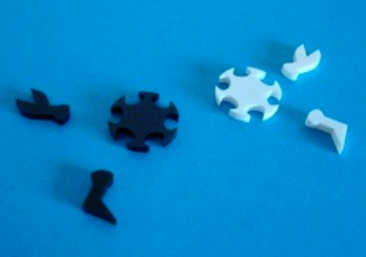
\includegraphics[width=0.20\textwidth]{adaptoidsDissecados}
    	\caption{Corpo e membros de um "adaptoid"}
\end{wrapfigure}

Cada turno divide-se em 3 fases distintas, sendo elas, movimento, crescimento e alimentação. Durante a fase de movimento o jogador pode mover um dos seus “adaptoids”, o número de espaços percorridos depende do número de pernas desse “adaptoid”.

Não é possível mover o adaptoid através de espaços que estejam ocupados, apenas é possível mover em direção a espaços vazios sem obstáculos e mover para o topo de um “adaptoid” oposto, para iniciar a captura. Na fase de crescimento o jogador pode optar por um de dois casos possíveis, ou cria um novo corpo adjacente a um dos seus “adaptoids” existentes, ou então adiciona uma perna, ou garra, a um dos seus “adaptoids” existentes no tabuleiro. Na fase de alimentação, é verificada em cada peça do inimigo se ela está com fome, ou seja, o número  de espaços vazios à sua volta terá que ser igual ou maior ao número de membros do “adaptoid”. No caso de fome, a peça inimiga morre, é removida e é atribuído um ponto ao jogador. Durante a captura o “adaptoid ”com mais garras ganha e o “adaptoid ” derrotado é removido do tabuleiro. Em caso do número de garras dos “adaptoids” ser igual, ambos são removidos e cada jogador recebe um ponto. As peças de “adaptoids” mortos poderão ser novamente usadas. O jogo termina quando um jogador chega aos 5 pontos ou quando um dos jogadores ficar sem nenhum “adaptoid” no tabuleiro.


\begin{figure}[h]
    \begin{center}
        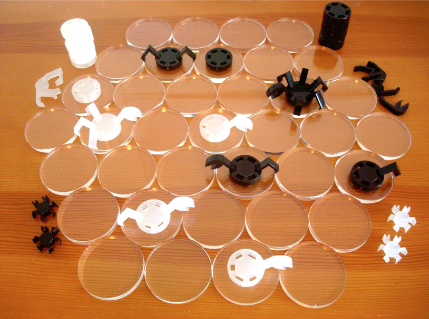
\includegraphics[scale=0.5]{jogoDecorrer}
        \caption{Estado de um jogo de adaptoid}
        \centering
    \end{center}
\end{figure}

\newpage
%%%%%%%%%%%%%%%%%%%%%%%%%%
\section{Lógica do Jogo}

\subsection{Representação do Estado do Jogo}  Para representar o tabuleiro do jogo optámos por uma lista de listas, onde cada uma das listas define uma das linhas do tabuleiro e por consequência cada elemento dessa lista representa uma célula no nosso jogo,  para facilitar a pesquisa de casas adjacentes foi inserido no início de cada lista alguns átomos que mais tarde serão interpretados como espaços por forma a garantir a forma hexagonal definida pelos criadores do jogo. As peças do jogo, os “adaptoids”, são representados usando uma lista de 4 elementos ([Id,Cor,NPernas,NGarras]). Os ID têm como função facilitar na pesquisa das peças no tabuleiro. A Cor assume o valor ‘O’(white) ou ‘X’(black), e representa o jogador ao qual a peça pertence, uma vez que na consola do sicstus não é possível alterar a cor. O NPernas como o nome indica é o número de pernas que a peça possui, idem para o NGarras.

\begin{figure}[h]
    \begin{center}
        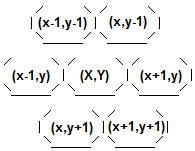
\includegraphics[scale=0.5]{posicoesRelativas}
        \caption{Posições relativas a uma célula central}
        \centering
    \end{center}
\end{figure}
Nota: Os átomos ‘a’,’b’,’c’,'d','e','f','g' e ‘\#’ são usados para controlar a posição das casas do jogo relativa à lista que representa a linha do tabuleiro onde estas se encontram, ou seja, com a introdução destes símbolos é possível seguir a seguinte lógica: Para uma determinada célula na posição (x,y), a célula-vizinha imediatamente abaixo do lado esquerdo está na posição (x,y+1) e a célula imediatamente abaixo do lado direito está na posição (x+1,y+1). Neste pequeno exemplo, o jogador da equipa ‘X’(white) ganhou porque o jogador da equipa ‘O’(black) não possui mais nenhuma peça no tabuleiro. Também é possível ambos os jogadores terem peças no tabuleiro e um ganhar, mas neste caso o jogador vencedor alcançou primeiro os 5 pontos.



\newpage

\subsection{Visualização do Tabuleiro} Originalmente as células do tabuleiro são redondas, mas para efeitos de visualização utilizando caracteres ASCII, estas são representadas como hexágonos. Com este formato, para ser possível o desenho do “adaptoid” contendo as suas garras e pernas seguiu-se a seguinte estratégia: Nesta célula é possível observar todas as posições possíveis para as garras(símbolo Y ) e pernas(símbolo L), este caso é impossível já que o número máximo de membros é 6, mas para efeitos de demonstração do funcionamento, é possível observar que as garras(Y) são desenhadas apenas no topo e no meio (caso sejam 6 garras no total), o mesmo acontece para as pernas. O símbolo B representa a cor do “adaptoid” e à sua volta está o número dessa peça.
Para que o desenho de cada célula seja possível, para cada linha do conteúdo do tabuleiro são desenhadas 4 linhas no ecrã, sendo elas:

\begin{table}[h!]
  \centering
  \caption{Legenda das camadas de uma célula.}
  \label{tab:table1}
 \newcolumntype{P}[1]{>{\centering\arraybackslash}p{#1}}
  \begin{tabular}{ c |  P{9.8cm}}
	\hline &
	\\
	
\includegraphics[width=0.1\textwidth]{topo}
           & A linha de topo que contém o número de garras (até 5 garras).
	\\&
	\\

	
\includegraphics[width=0.1\textwidth]{meio}
	& A linha do meio que contém o sexto membro (garra/perna), a cor e  número da peça.
	\\

	
\includegraphics[width=0.1\textwidth]{baixo}
	& A linha de baixo que contém o número de pernas (até 5 pernas).

	\\
	
\includegraphics[width=0.06\textwidth]{separacao}
	& A linha de separação para ser possível uma melhor distinção entre células adjacentes.
	\end{tabular}
\end{table}
\FloatBarrier
Foram utilizados símbolos especiais que apenas são usados como espaçamento, para que seja possível enquadrar as células no seu local. O predicado de visualização já se encontra 100\% desenvolvido sendo que recebe um tabuleiro no formato de lista de listas e procede ao desenho no mesmo na consola como se pode ver na figura ao lado.

\subsection{Lista de Jogadas Válidas}Foram implementados predicados que definem as jogadas válidas, estes predicados implementam as jogadas propriamente ditas e validam no caso do utilizador, no caso do computador são usados para obter a lista de jogadas possíveis. As três regras que se seguem dizem respeito às diferentes fases de que cada jogada (Movimento(M), Evolução(E) e Alimentação(famintos)).
\begin{itemize}
    \item \textit{lerRegraM(+Cor,+Acao,+JogoInicial,-JogoFinal)} , as ações possíveis incluem \textit{mover(+X,+Y,+Ori)} e \textit{capturar(+X,+Y,+Ori)}.
    \item \textit{lerRegraE(+Cor,+Acao,+JogoInicial,-JogoFinal)} , as ações incluem \textit{aP(+X,+Y)} para adicionar uma perna, \textit{aG(+X,+Y)} para adicionar uma garra e \textit{aC(+X,+Y,+Ori)} para adicionar um novo adaptoid.
    \item \textit{famintos(+JogoInicial,+Cor,-JogoFinal)}.
\end{itemize}

\newpage

\subsection{Execução de Jogadas} Validação e execução de uma jogada num tabuleiro, obtendo o novo estado do jogo. Exemplo: \textit{move(+Move, +Board, -NewBoard)}.
\begin{itemize}
    \item \textit{capturar(+JogoInicial, +ID, +Cor, +Ori, -JogoFinal)}.
    \item \textit{moverPeca(+JogoInicial, +ID, +Cor, +Ori, -JogoFinal)}.
    \item \textit{addPerna(+Board, +Cor, +ID, -NewBoard)}.
    \item \textit{addGarra(+Board, +Cor, +ID, -NewBoard)}.
    \item \textit{addCorpo(+Board, +ID, +Cor, +Ori, -NewBoard)}.
    \item \textit{esfomeados(+OriginalBoard, +BoardCopy, +Cor, -Nremovidos, -NewBoard)} esta função não é usada diretamente pelo utilizador mas é feita no final de cada jogada.
\end{itemize}

\subsection{Avaliação do Tabuleiro}\label{evalTab}

A avaliação do estado do jogo é realizada no predicado  \textit{getValue(+JogoI, +Cor,+Pos, -Value)}, este predicado internamente usa outros predicados de avaliação, para que promova certos movimentos. Estes predicados são:

\begin{itemize}
    \item \textit{getValueByPoints(+JogoI, +Cor, +Pos, -Value, +M)}. Atribui um valor dependendo os pontos ganhos nessa jogada, sendo M a pontuação.
    \item \textit{getValueByPecas(+JogoI, +Cor, +Pos, -Value, +M)}. Atribui um valor dependendo do número de peças , sendo M a pontuação.
    \item \textit{getValueByStarving(+JogoI, +Cor, +Pos, -Value, +M)}. Atribui um valor dependendo do número de peças que possam ser perdidas posteriormente devido à condição de fome, sendo M a pontuação.
    \item \textit{getValueByPernas(+JogoI, +Cor, +Pos, -Value, +M1, +M2)}. Atribui um valor dependendo do número de garras e o número de adaptoids com garras, sendo M1 a pontuação de elementos com pernas e M2 o numero total de pernas.
    \item \textit{getValueByGarras(+JogoI, +Cor, +Pos, -Value, +M1, +M2)}. Atribui um valor dependendo do número de garras e o número de adaptoids com garra, sendo M1 a pontuação de elementos com garras e M2 o numero total de garras.
    \item \textit{getValueByMovimento(+JogoI, +Cor, +Pos, -Value, +M)}. Atribui um valor dependendo do número de pernas e o número de adaptoids com pernas, sendo M a pontuação.
    \item \textit{getValueByCloser(+JogoI, +Cor, +Pos, -Value, +M)}. Atribui um valor dependendo da próximidade e possibilidade de ataque a um inimigo, sendo M a pontuação.
\end{itemize}

\subsection{Final do Jogo} Foi criado o predicado \textit{ganhou(-Jogador,+Jogo)} que avalia se um dado jogo chegou ao fim, verificando as seguintes condições : algum dos jogadores alcançou os 5 pontos ou algum dos jogadores não possuí peças no tabuleiro. Este predicado é chamado em duas ocasiões, a primeira, no fim de cada jogada simplesmente para saber se o jogo terminou, ou seja, se existe um vencedor, e uma segunda vez após ter terminado o \textit{loop} de jogar para se obter o estado de terminação (jogador vencedor ou empate) de forma a imprimir o resultado.

\subsection{Jogada do Computador}
A escolha da melhor jogada é feita no predicado:
\begin{itemize}
	\item \textit{escolheMelhorJogada(+JogoI,+Cor,+Modo,-JogoF)}.
\end{itemize}

O modo determina o nível de dificuldade do computador, tendo como opções disponíveis um modo de ataque (\textit{op}) e um modo de defesa (\textit{notOP}). Internamente o modo alterna entre \textit{getValue} e \textit{getValue2} que apenas mudam os multiplicadores para obter comportamentos diferentes. A forma como são escolhidas as opções já foi mencionada na secção~\ref{evalTab}.

\subsection{Testes}

Foram realizados testes durante a fase de desenvolvimento da lógica do jogo, para garantir a funcionalidade dos predicados implementados e o cumprimento das regras.

Estes testes apenas abrangem a parte lógica do projeto uma vez que é considerada como sendo a componente mais critica do projeto. O que implica que terá de ser, por conseguinte, a parte mais robusta.


%%%%%%%%%%%%%%%%%%%%%%%%%%
\newpage
\section{Interface com o Utilizador}

O módulo de interface principal divide-se em vários predicados sendo que cada um indica um menu. Este design foi desenvolvido a pensar no utilizador, para que seja possivel uma navegação mais intuitiva entre os menus.
\begin{figure}[h]
    \begin{minipage}[b]{0.4\textwidth}
        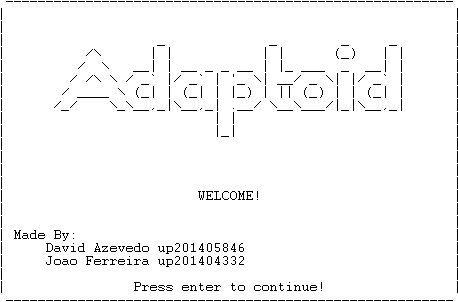
\includegraphics[scale=0.5]{menuPrincipal}
        \caption{Menu de início.}
    \end{minipage}
    \begin{minipage}[b]{0.4\textwidth}
        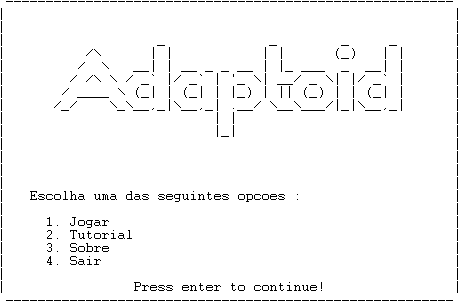
\includegraphics[scale=0.5]{menuEscolha}
        \caption{Menu principal.}
    \end{minipage}
\end{figure}


Os menus que o utilizador pode encontrar contêm:

\begin{itemize}
	\item Instruções (tutorial).
	\item Especificação do jogo.
	\item Escolha do tipo de jogo.
	\item Escolha da dificuldade do computador.
\end{itemize}

\begin{figure}[h]

    	\centering
     	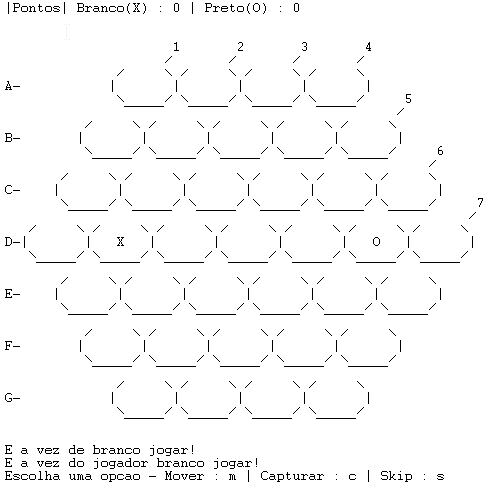
\includegraphics[scale=0.5]{ingame1}
	\caption{Menu de jogo.}
	\label{fig:figuramenu}

\end{figure}
No modo humano contra humano ou humano contra computador, durante a jogada do utilizador, é apresentado um menu como o indicado na figura~\ref{fig:figuramenu}, indicando os passos que o utilizador deverá seguir para realizar a sua jogada.

Em modo computador contra computador, é apresentado ao utilizador o tabuleiro do resultado de cada ronda, sendo necessária a interação do utilizador para proceder à próxima ronda, terminando com um texto indicativo do resultado final.



%%%%%%%%%%%%%%%%%%%%%%%%%%
\newpage
\section{Conclusões}
O grupo vê positivamente o resultado final que obteve e os conhecimentos adquiridos durante o desenvolvimento do projeto. Reconhecemos que a linguagem Prolog é bastante útil para a resolução de problemas relacionados com lógica, como era o caso deste mesmo jogo de tabuleiro, entre outros problemas do mundo real. Nunca é demais lembrar o peso e o significado destes problemas, uma vez que o modelo estrutural aqui representado pode-nos levar a considerar a reestruturação dos modos de operação convencionais.
\\

O jogo Adaptoid mostrou-nos que apesar da sua simplicidade consegue ser um jogo bastante apelativo e um bom exercício cerebral.
\\

Foram encontradas algumas dificuldades durante a realização deste trabalho que com o auxilio do material disponibilizado pelos docentes, e ainda o material que se encontra online, foram possiveis de ser ultrapassados. Inicialmente não foi um projeto que nos apelou muito devido a ser um estilo "relativamente" novo de programação e ao qual não estamos habituados, isto significa que, durante os primeiros dias de impletamentação o grupo esteve um pouco perdido e sem saber o que fazer. Optámos por utilizar uma tarde somente na pesquisa de informação sobre o Prolog (de notar que este tempo foi reduzido devido às informações e dicas já apresentadas nas aulas teóricas). Após este periodo de adaptação, os estudantes conseguiram resolver o problema proposto de uma forma ágil, dedicada, empenhada e acima de tudo correta.
\\

Na nossa opinião, é importante referir que o modo de \textit{input} não ficou da forma que o grupo mais gostaria, mas uma vez que é necessário tratar situações de erro humano achamos que a opção escolhida, apesar de não ser a mais funcional, é a mais robusta. Outro aspeto importante é a inteligência artificial, mas esta parte não recebeu uma importância tão elevada devido a ser alvo de estudo no próximo semestre.
\\

Concluindo, foi um projeto bastante interessante e educativo que nos abriu novos horizontes no mundo da programação em lógica, ambos os estudantes estão gratos pela experência e orgulhosos pelo seu resultado.

\clearpage

\nocite{*}
\addcontentsline{toc}{section}{Bibliografia}
\renewcommand\refname{Bibliografia}
\bibliographystyle{plain}
\bibliography{referencia}{}

\newpage
\appendix
\section{Anexos}
\subsection{adaptoid.pl}
\begin{lstlisting}
:- use_module(library(lists)).
:- include('tabuleiro.pl').
:- include('testes.pl').
:- include('logic.pl').
:- include('utils.pl').
:- include('ai.pl').
:- include('menu.pl').

%Predicado que inicia o jogo criando um tabuleiro com as posicoes iniciais e a instancia jogo com ambos os pontos a 0 e o novo tabuleiro criado
init :- write('Comecando o jogo!'),tabuleiro(Tab), asserta(jogo(0,0,Tab)), nl.

%Predicado para terminar e eliminar a instancia de jogo
end :- retract(jogo(_,_,_)), write('Fim do Jogo!'), nl.

%Predicados de desenho do jogo
desenharJogo(A,B,Tab) :- clearScreen, write('|Pontos| Branco(X) : '), write(A), write(' | Preto(O) : '), write(B), nl, desenharTabuleiro(Tab).
desenharJogo(jogo(A,B,Tab)) :- desenharJogo(A,B,Tab).

%Predicados para imprimir o resultado do jogador
imprimeVencedor(branco):- write('Jogador Branco Ganhou! Parabens!'), nl.
imprimeVencedor(preto):- write('Jogador Preto Ganhou! Parabens!'), nl.
imprimeVencedor(empate):- write('Ninguem Ganhou! Empate!'), nl.
imprimeVez(Cor):- write('E a vez do jogador '), write(Cor), write(' jogar!'), nl.

%Predicado para a jogada do jogador branco
jogadaBranco(Jogo,Jogo) :- ganhou(_,Jogo).
jogadaBranco(jogo(A,B,Tab),jogo(A1,B1,T1)) :- desenharJogo(A,B,Tab), write('E a vez de branco jogar!'), nl, jogada(jogo(A,B,Tab),branco,jogo(A1,B1,T1)).

%Predicado para a jogada do jogador preto
jogadaPreto(Jogo,Jogo) :- ganhou(_,Jogo).
jogadaPreto(jogo(A,B,Tab),jogo(A1,B1,T1)) :- desenharJogo(A,B,Tab), write('E a vez de preto jogar!'), nl, jogada(jogo(A,B,Tab),preto,jogo(A1,B1,T1)).

%Predicados que representam uma ronda do jogo
jogando(hh,Jogo) :- retract(jogo(A,B,Tab)), !, jogadaBranco(jogo(A,B,Tab),jogo(A1,B1,T1)), !, jogadaPreto(jogo(A1,B1,T1),jogo(A2,B2,T2)), asserta(jogo(A2,B2,T2)), Jogo = jogo(A2,B2,T2).
jogando(hh,_).
jogando(hOp,Jogo) :- jogando(hc,op,Jogo).
jogando(hRe,Jogo) :- jogando(hc,notOp,Jogo).
jogando(opOp,Jogo):- jogando(cc,Jogo,op,op).
jogando(opRe,Jogo):- jogando(cc,Jogo,op,notOp).
jogando(reRe,Jogo):- jogando(cc,Jogo,notOp,notOp).
jogando(hc,M,Jogo) :- retract(jogo(A,B,Tab)), !, jogadaBranco(jogo(A,B,Tab),jogo(A1,B1,T1)), !, jogadaComputador(preto,M,jogo(A1,B1,T1),jogo(A2,B2,T2)), desenharJogo(A2,B2,T2), asserta(jogo(A2,B2,T2)), Jogo = jogo(A2,B2,T2).
jogando(hc,_,_).
jogando(cc,Jogo,M1,M2) :- retract(jogo(A,B,Tab)), !, jogadaComputador(branco,M1,jogo(A,B,Tab),jogo(A1,B1,T1)), jogadaComputador(preto,M2,jogo(A1,B1,T1),jogo(A2,B2,T2)), desenharJogo(A2,B2,T2), write('Prima /*|ENTER|*\\'), get_char(_), asserta(jogo(A2,B2,T2)), Jogo = jogo(A2,B2,T2).
jogando(cc,_,_,_).

%Loop do Jogo
jogar(Modo) :- init, repeat, once(jogando(Modo,Jogo)), ganhou(Jogador,Jogo), desenharJogo(Jogo), imprimeVencedor(Jogador), end.

%Representa uma jogada individual
jogada(jogo(A,B,Tab),Cor,jogo(A3,B3,T3)):-  imprimeVez(Cor), !, repeat, movimento(jogo(A,B,Tab),Cor,jogo(A1,B1,T1)), desenharJogo(A1,B1,T1), !, repeat, evoluir(jogo(A1,B1,T1),Cor,jogo(A2,B2,T2)), !, famintos(jogo(A2,B2,T2),Cor,jogo(A3,B3,T3)).

%Predicado para ler a opcao de movimento
movimento(JI,Cor,JF) :- write('Escolha uma opcao - Mover : m | Capturar : c | Skip : s'), nl, !, read(X), acao1(JI,X,Regra), !, lerRegraM(Cor,Regra,JI,JF).
lerRegraM(_,s,Jogo,Jogo).
lerRegraM(Cor,mover(X,Y,Ori),jogo(A,B,Tab),jogo(A,B,T1)) :- getSimboloXY(Tab,[ID,Cor,_,P],X,Y), P > 0, validarOri(Ori,P), moverPecaLista(Tab,ID,Cor,Ori,T1).
lerRegraM(Cor,capturar(X,Y,Ori), jogo(A,B,Tab), JF) :-  getSimboloXY(Tab,[ID,Cor,G,_],X,Y), G > 0, capturar(jogo(A,B,Tab),ID,Cor,Ori,JF).

%Predicado para ler a opcao de evolucao
evoluir(Jogo,_,Jogo):- ganhou(_,Jogo).
evoluir(JI,Cor,JF) :-   write('Escolha um opcao - Adicionar Perna : p | Adicionar Garra : g | Adicionar Corpo : c | Skip : s'), nl , !, read(Acao), acao2(Acao,Regra), !, lerRegraE(Cor,Regra,JI,JF).
lerRegraE(_,s,Jogo,Jogo).
lerRegraE(Cor,aP(X,Y),jogo(A,B,Tab),jogo(A,B,T1)):- getSimboloXY(Tab,[ID,Cor,G,P],X,Y) , (P + G) < 6 , addPerna(Tab,Cor,ID,T1).
lerRegraE(Cor,aG(X,Y),jogo(A,B,Tab),jogo(A,B,T1)):- getSimboloXY(Tab,[ID,Cor,G,P],X,Y) , (P + G) < 6 , addGarra(Tab,Cor,ID,T1).
lerRegraE(Cor,aC(X,Y,Ori),jogo(A,B,Tab),jogo(A,B,T1)):- getSimboloXY(Tab,[ID,Cor,_,_],X,Y) , addCorpo(Tab,ID,Cor,Ori,T1).

%Predicado para a fase de alimentacao
famintos(Jogo,_,Jogo):- ganhou(_,Jogo).
famintos(jogo(A,B,T),Cor,jogo(A1,B1,T1)) :- corInv(Cor,CI), removeEsfomeados(T,CI,Removidos,T1), somarPontos(Cor,A,B,A1,B1,Removidos).

%Predicados que consuante as pernas da peca do jogador pede uma movimentacao individual
lerOris(0,[]).
lerOris(Npernas,OriList) :- write('Restam-lhe '), write(Npernas), write(' movimento(s), indique uma orientacao[0...5] \'s\' para sair '), read(Ori), (Ori = 's' -> OriList = []; (oriDic(Ori,_,_), N1 is Npernas - 1, lerOris(N1,L), OriList = [Ori|L])).

%Predicado de verificacao de uma jogada valida na fase do movimento
acao1(jogo(_,_,Tab),m,Regra):-  lerPosicao(X,Y), getSimboloXY(Tab,[_,_,_,P],X,Y), lerOris(P,OriList), Regra = mover(X,Y,OriList).
acao1(_,c,Regra):-  lerPosicao(X,Y), write('Indique uma orientacao [0..5]'), read(Ori), oriDic(Ori,_,_), Regra = capturar(X,Y,Ori).
acao1(_,s,s).
acao1(_,_,_) :- invalido.

%Predicado de verificacao de uma jogada valida na fase do evolucao
acao2(p,Regra) :- lerPosicao(X,Y), Regra = aP(X,Y).
acao2(g,Regra) :- acao2(p,aP(X,Y)), Regra = aG(X,Y).
acao2(c,Regra) :- acao2(p,aP(X,Y)), write('Indique uma orientacao [0..5]'), read(Ori), oriDic(Ori,_,_), Regra = aC(X,Y,Ori).

acao2(s,s).
acao2(_,_) :- invalido.
invalido :- write('Opcao Invalida!'), nl, fail.
\end{lstlisting}

\subsection{ai.pl}
\begin{lstlisting}
/*Predicado que realiza uma jogada do computador dependendo do seu modo de jogo*/
jogadaComputador(Cor,Modo,jogo(A,B,Tab),JogoF) :- desenharJogo(A,B,Tab), nl, imprimeVez(Cor), !, escolheMelhorJogada(jogo(A,B,Tab), Cor,Modo, JogoF).

/*Predicado que retorna um jogo para uma determinada cor*/
jogadaBot(JogoI,Cor,JogoF) :- lerRegraM(Cor,_,JogoI,J1), lerRegraE(Cor,_,J1,J2), famintos(J2,Cor,JogoF).

/*Predicado que escolhe a melhor jogada*/
escolheMelhorJogada(JogoI,Cor,Modo,JogoF):- findall(Jogo,jogadaBot(JogoI,Cor,Jogo),Possibilidades), avaliarJogada(JogoI,Cor,Possibilidades,Modo,JogoF).

/*Predicados que avaliam a melhor jogada dependendo do modo de jogo*/
avaliarJogada(JI,C,P,op,J) :- avaliarJogadaOp(JI,C,P,_,J).
avaliarJogada(JI,C,P,notOp,J) :- avaliarJogadaNotOp(JI,C,P,_,J).

/*Predicados que avaliam o melhor tabuleiro*/
melhorTabuleiro(J1,N1,_,N2,J1,N1) :- N1 > N2, !.
melhorTabuleiro(_,_,J2,N2,J2,N2).

/*Predicados que devolve pontuacao dependendo do numero de pontos efectuados*/
getValueByPoints(jogo(_,_,_),branco,jogo(5,_,_),100,_).
getValueByPoints(jogo(_,_,_),preto,jogo(_,5,_),100,_).
getValueByPoints(jogo(A,B,_),branco,jogo(A1,B1,_),Value,M) :- Adif is A1 - A, Bdif is B1 - B, V1 is Adif - Bdif, Value is V1 * M.
getValueByPoints(jogo(A,B,_),preto,jogo(A1,B1,_),Value,M) :- Adif is A1 - A, Bdif is B1 - B, V1 is Bdif - Adif, Value is V1 * M.

/*Predicados que devolve pontuacao dependendo do numero de pecas*/
getValueByPecas(_, Cor, Pos, 100,_):-  corInv(Cor, CorOponente), getPecasByCor(Pos,CorOponente,0).
getValueByPecas(JogoI, Cor, Pos, Value,M):- getPecasByCor(JogoI,Cor,PecasInicial), !, getPecasByCor(Pos,Cor,PecasFinal), !, V1 is PecasFinal - PecasInicial, ((V1 > 0, PecasFinal == M) -> Value is 10; (V1 > 0, PecasFinal < M) -> Value is 10; (V1 < 0, PecasFinal == M) -> Value is 0; (V1 < 0, PecasFinal < M) -> Value is -5; Value is -10).

/*Predicado que devolve pontuacao dependendo do numero de pecas a morrer a fome*/
getValueByStarving(_,Cor,Pos,Value,M):- getStarvingNum(Pos,Cor,Res), V1 is 0 - Res, Value is V1 * M.

/*Predicado que devolve pontuacao dependendo do numero de pernas*/
getValueByPernas(_,Cor,Pos,Value,M1,M2):- getPernaNum(Pos,Cor,V1,Res), V2 is V1 * M1, V3 is Res * M2, Value is V2 + V3.

/*Predicado que devolve pontuacao dependendo do numero de garras*/
getValueByGarras(_,Cor,Pos,Value,M1,M2):-   getGarraNum(Pos,Cor,V1,Res), V2 is V1 * M1, V3 is Res * M2, Value is V2 + V3.

/*Predicados que devolve pontuacao dependendo de movimento ocorrido*/
getValueByMovimento(jogo(_,_,T1), Cor, jogo(_,_,T2), M,M):- getMoveu(T1,T2,Cor,N), N > 0, !.
getValueByMovimento(_, _, _, -10,_).

/*Predicados que devolve pontuacao dependendo de aproximacao ao inimigo*/
getValueByCloser(jogo(_,_,Tab),Cor,jogo(_,_,Pos),M,M):- corInv(Cor,CorInimigo), findall(IDinimigo,(getSimboloXY(Tab,[IDinimigo,CorInimigo,GI,_],XInimigo,YInimigo), getSimboloXY(Tab,[ID,Cor,_,_],Xinicial,Yinicial), getSimboloXY(Pos,[ID,Cor,GF,_],Xfinal,Yfinal), GF >= GI, dist(XInimigo,YInimigo,Xinicial,Yinicial,DistInicial), dist(XInimigo,YInimigo,Xfinal,Yfinal,DistFinal), DistFinal < DistInicial),Elems), length(Elems,Res), Res > 0.
getValueByCloser(_,_,_,-10,_).

/*Predicados que devolvem pontuacao total do tabuleiro*/
getValue(JogoI,Cor,Pos,Value):- getValueByPoints(JogoI,Cor,Pos,V1,15), getValueByPecas(JogoI,Cor,Pos,V2,3), getValueByStarving(JogoI,Cor,Pos,V3,50), getValueByPernas(JogoI,Cor,Pos,V4,5,10), getValueByGarras(JogoI,Cor,Pos,V5,5,10), getValueByMovimento(JogoI,Cor,Pos,V6,10), getValueByCloser(JogoI,Cor,Pos,V7,100), somarLista([V1,V2,V3,V4,V5,V6,V7],Value).
getValue2(JogoI,Cor,Pos,Value):- getValueByPoints(JogoI,Cor,Pos,V1,15), getValueByPecas(JogoI,Cor,Pos,V2,5), getValueByStarving(JogoI,Cor,Pos,V3,-1), getValueByPernas(JogoI,Cor,Pos,V4,10,15), getValueByGarras(JogoI,Cor,Pos,V5,10,15), getValueByMovimento(JogoI,Cor,Pos,V6,10), getValueByCloser(JogoI,Cor,Pos,V7,-20), somarLista([V1,V2,V3,V4,V5,V6,V7],Value).

/*Predicadoss que avaliam a melhor jogada no momento*/
avaliarJogadaOp(JogoI,_,[],-2000,JogoI).
avaliarJogadaOp(JogoI,Cor,[Pos|Possibilidades],N,JogoF) :- avaliarJogadaOp(JogoI,Cor,Possibilidades,N1,J1), getValue(JogoI,Cor,Pos,Value), melhorTabuleiro(J1,N1,Pos,Value,JogoF,N).
avaliarJogadaNotOp(JogoI,_,[],-2000,JogoI).
avaliarJogadaNotOp(JogoI,Cor,[Pos|Possibilidades],N,JogoF) :- avaliarJogadaNotOp(JogoI,Cor,Possibilidades,N1,J1), getValue2(JogoI,Cor,Pos,Value), melhorTabuleiro(J1,N1,Pos,Value,JogoF,N).
\end{lstlisting}

\subsection{logic.pl}
\begin{lstlisting}
/*Adicionar um Garra a um adaptoid*/
addGarraAux([],_,_,[]).
addGarraAux([[ID,Cor,G,P] | T],Cor, ID, Tr) :- G1 is G + 1, !, validaPeca(G1,P), Tr = [[ID,Cor,G1,P]|T].
addGarraAux([A|T],Cor,ID,Tr) :- addGarraAux(T,Cor,ID,T1), Tr = [A|T1].
addGarra([],_,_,[]).
addGarra([A|T],Cor,ID,Tr) :- addGarraAux(A,Cor,ID,LN1), addGarra(T,Cor,ID,LN2), Tr = [LN1|LN2].

/*Adicionar uma Perna a um adaptoid*/
addPernaAux([],_,_,[]).
addPernaAux([[ID,Cor,G,P] | T],Cor, ID, Tr) :- P1 is P + 1, !, validaPeca(G,P1), Tr = [[ID,Cor,G,P1]|T].
addPernaAux([A|T],Cor,ID,Tr) :- addPernaAux(T,Cor,ID,T1), Tr = [A|T1].
addPerna([],_,_,[]).
addPerna([A|T],Cor,ID,Tr) :- addPernaAux(A,Cor,ID,LN1), addPerna(T,Cor,ID,LN2), Tr = [LN1|LN2].

/*Predicados para verificar e remover os adaptoids que nao estam alimentados*/
vizinhoVazio(T,X,Y,OffSetX,OffSetY,Res) :-
X1 is X + OffSetX, Y1 is Y + OffSetY,
length(T,NL), Y1 < NL, nth0(Y1,T,LTemp),
length(LTemp,CL), X1 < CL, !,
getSimboloXY(T,Simb,X1,Y1),
isVazio(Simb, Res), !.
vizinhoVazio(_,_,_,_,_,0).

contaVazios(T,X,Y,Res) :-
vizinhoVazio(T,X,Y,-1,-1,R1), vizinhoVazio(T,X,Y,0,-1,R2),
vizinhoVazio(T,X,Y,-1,0,R3), vizinhoVazio(T,X,Y,1,0,R4),
vizinhoVazio(T,X,Y,0,1,R5), vizinhoVazio(T,X,Y,1,1,R6),
somarLista([R1,R2,R3,R4,R5,R6],Res).

esfomeado(T,A,Cor,B,C) :-   Max is B + C,!,
getSimboloXY(T,[A,Cor,B,C],X,Y),
contaVazios(T,X,Y,Res), !, Res < Max.
esfomeadosAux(_,[],_,0,[]).

esfomeadosAux(Tab,[[A,Cor,B,C] | Ls], Cor, N, Tr):-
esfomeado(Tab,A,Cor,B,C), !,
esfomeadosAux(Tab, Ls, Cor, Nr, Tm),
N is Nr + 1, Tr = [vazio | Tm ] .

esfomeadosAux(Tab,[A|Ls],Cor,N, [A|Tr]) :- esfomeadosAux(Tab,Ls,Cor,N,Tr).
esfomeados(_,[],_,0,[]).
esfomeados(Tab,[L|T], Cor, N, Tr):-
esfomeadosAux(Tab, L, Cor, N1, Lr),
esfomeados(Tab,T, Cor, N2, T1),
N is N1 + N2, Tr = [Lr | T1].

removeEsfomeados(Tab,Cor,N,Tr) :- esfomeados(Tab,Tab,Cor,N,Tr).

/*Verificar se uma movimentacao e possivel*/
checkMov(Tab,ID,Cor,Ori,X,Y,Peca):-
oriDic(Ori,Ox,Oy),
getSimboloXY(Tab,[ID,Cor,_,_],Xatual,Yatual), !,
vizinhoVazio(Tab,Xatual,Yatual,Ox,Oy,Res), Res is 1, !,
getSimboloXY(Tab,Peca,Xatual,Yatual),
X is Xatual + Ox, Y is Yatual + Oy.

/*Remover uma peca da tabuleiro*/
removePecaAux([],_,_,[]).
removePecaAux([[ID,Cor,_,_]|Line],ID,Cor,[vazio|Res]):- removePecaAux(Line,ID,Cor,Res), !.
removePecaAux([Elem|Line],ID,Cor,[Elem|Res]):- removePecaAux(Line,ID,Cor,Res).
removePeca([],_,_,[]).
removePeca([Line|Tab],ID,Cor,Res):-
removePecaAux(Line,ID,Cor,LineRes),
removePeca(Tab,ID,Cor,LineRes2),
Res = [LineRes|LineRes2].

/*Inserir uma peca num tabuleiro*/
inserePecaAux([],_,_,[]).
inserePecaAux([_|Line],Peca,CoordX,LineRes) :-
CoordX is 0,
LineRes = [Peca|Line].
inserePecaAux([Elem|Line],Peca,CoordX,[Elem|LineRes]) :-
NewX is CoordX - 1,
inserePecaAux(Line,Peca,NewX,LineRes).
inserePeca([],_,_,_,[]).
inserePeca([Line|Res],Peca,CoordX,CoordY,TabRes) :-
CoordY is 0,
inserePecaAux(Line,Peca,CoordX,NewLine), !,
TabRes = [NewLine|Res].
inserePeca([Line|Res],Peca,CoordX,CoordY,[Line|TabRes]):-   NewY is CoordY - 1,
inserePeca(Res,Peca,CoordX,NewY,TabRes).

/*Mover um peca*/
moverPecaLista(Tab,_,_,[],Tab).
moverPecaLista(Tab,ID,Cor,[Ori|Os],T1) :- oriDic(Ori,_,_), moverPeca(Tab,ID,Cor,Ori,T2), moverPecaLista(T2,ID,Cor,Os,T1).

moverPeca(Tab,ID,Cor,Ori,TabRes) :-
checkMov(Tab,ID,Cor,Ori,CoordX,CoordY,Peca),
removePeca(Tab,ID,Cor,Res),
inserePeca(Res,Peca,CoordX,CoordY,TabRes).

/*Predicados para atacar e capturar um inimigo*/
maisGarras(jogo(A,B,Tab),G1,G2,ID1,Cor1,ID2,Cor2,Ori,jogo(A1,B1,TabRes)):-
G1 > G2, !,
removePeca(Tab,ID2,Cor2,Res),
moverPeca(Res,ID1,Cor1,Ori,TabRes),
somarPontos(Cor1,A,B,A1,B1,1).

maisGarras(jogo(A,B,Tab),G1,G2,ID1,Cor1,_,Cor2,_,jogo(A1,B1,TabRes)):-
G2 > G1, !,
removePeca(Tab,ID1,Cor1,TabRes),
somarPontos(Cor2,A,B,A1,B1,1).

maisGarras(jogo(A,B,Tab),G1,G2,ID1,Cor1,ID2,Cor2,_,jogo(A1,B1,TabRes)):-
G1 is G2, G1 > 0, !,
removePeca(Tab,ID1,Cor1,Res),
removePeca(Res,ID2,Cor2,TabRes),
somarPontos(Cor1,A,B,A2,B2,1),
somarPontos(Cor2,A2,B2,A1,B1,1).

atacar(jogo(A,B,Tab),ID1,Cor1,ID2,Cor2,Ori,jogo(A1,B1,TabRes)) :- getSimboloXY(Tab,[ID1,Cor1,G1,_],_,_), getSimboloXY(Tab,[ID2,Cor2,G2,_],_,_), !, maisGarras(jogo(A,B,Tab),G1,G2,ID1,Cor1,ID2,Cor2,Ori,jogo(A1,B1,TabRes)).

capturar(jogo(A,B,Tab),ID,Cor,Ori,jogo(A1,B1,TabRes)):-
getSimboloXY(Tab,[ID,Cor,_,_],X,Y),
oriDic(Ori,Ox,Oy), NewX is X + Ox, NewY is Y + Oy,
getSimboloXY(Tab,[IDinimigo,CorInimigo,_,_],NewX,NewY),
Cor \= CorInimigo,
atacar(jogo(A,B,Tab),ID,Cor,IDinimigo,CorInimigo,Ori,jogo(A1,B1,TabRes)).

/*Adicionar um corpo de um adaptoid*/
vizinho(Tab,Cor,CoordX,CoordY) :- Y is CoordY - 1, getSimboloXY(Tab,[_,Cor,_,_],CoordX,Y).
vizinho(Tab,Cor,CoordX,CoordY) :- X is CoordX + 1, getSimboloXY(Tab,[_,Cor,_,_],X,CoordY).
vizinho(Tab,Cor,CoordX,CoordY) :- X is CoordX + 1, Y is CoordY + 1, getSimboloXY(Tab,[_,Cor,_,_],X,Y).
vizinho(Tab,Cor,CoordX,CoordY) :- Y is CoordY + 1, getSimboloXY(Tab,[_,Cor,_,_],CoordX,Y).
vizinho(Tab,Cor,CoordX,CoordY) :- X is CoordX - 1, getSimboloXY(Tab,[_,Cor,_,_],X,CoordY).
vizinho(Tab,Cor,CoordX,CoordY) :- X is CoordX - 1, Y is CoordY - 1, getSimboloXY(Tab,[_,Cor,_,_],X,Y).

canPlace(Tab,_,CoordX,CoordY):-   getSimboloXY(Tab,vazio,CoordX,CoordY).

addCorpo(Tab,ID,Cor,Ori,TabRes):-getSimboloXY(Tab,[ID,Cor,_,_],CoordX,CoordY), oriDic(Ori,Ox,Oy), NewX is CoordX + Ox, NewY is CoordY + Oy, canPlace(Tab,Cor,NewX,NewY), addCorpo2(Tab,Cor,NewX,NewY,TabRes).

addCorpo2(Tab,Cor,CoordX,CoordY,TabRes):- getNewIndex(Tab,Cor,0,ID), inserePeca(Tab,[ID,Cor,0,0],CoordX,CoordY,TabRes).
\end{lstlisting}

\subsection{menu.pl}
\begin{lstlisting}
clearScreen :- consuela(60).

consuela(0).
consuela(N):- nl, N1 is N - 1, consuela(N1).
sair.

lerPosicao(X,Y) :-  write('Indique a letra '), read(Cena), charDic(Cena,Y), write('Indique o numero '), read(X), nl.

adaptoidLogo :- write('|                                                        |'), nl,
write('|                                                        |'), nl,
write('|                   _             _        _     _       |'), nl,
write('|          /\\      | |           | |      (_)   | |      |'), nl,
write('|         /  \\   __| | __ _ _ __ | |_ ___  _  __| |      |'), nl,
write('|        / /\\ \\ / _` |/ _` | \'_ \\| __/ _ \\| |/ _` |      |'), nl,
write('|       / ____ \\ (_| | (_| | |_) | || (_) | | (_| |      |'), nl,
write('|      /_/    \\_\\__,_|\\__,_| .__/ \\__\\___/|_|\\__,_|      |'), nl,
write('|                          | |                           |'), nl,
write('|                          |_|                           |'), nl,
write('|                                                        |'), nl.

adaptoid :-  clearScreen,
write(' -------------------------------------------------------- '), nl,adaptoidLogo,
write('|                                                        |'), nl,
write('|                                                        |'), nl,
write('|                                                        |'), nl,
write('|                        WELCOME!                        |'), nl,
write('|                                                        |'), nl,
write('|                                                        |'), nl,
write('| Made By:                                               |'), nl,
write('|     David Azevedo up201405846                          |'), nl,
write('|     Joao Ferreira up201404332                          |'), nl,
write('|                                                        |'), nl,
write('|                Press enter to continue!                |'), nl,
write(' -------------------------------------------------------- '), nl,
            get_char(_), startMenu.

startMenu :-    clearScreen,
write(' -------------------------------------------------------- '), nl,adaptoidLogo,
write('|                                                        |'), nl,
write('|                                                        |'), nl,
write('|                                                        |'), nl,
write('|   Escolha uma das seguintes opcoes :                   |'), nl,
write('|                                                        |'), nl,
write('|     1. Jogar                                           |'), nl,
write('|     2. Tutorial                                        |'), nl,
write('|     3. Sobre                                           |'), nl,
write('|     4. Sair                                            |'), nl,
write('|                                                        |'), nl,
write('|                Press enter to continue!                |'), nl,
write(' -------------------------------------------------------- '), nl,
get_char(A), get_char(_),%How to tirar apenas um character de input
(A = '1' -> jogarMenu;
A = '2' -> tutorialMenu;
A = '3' -> aboutMenu;
A = '4' -> sair;
startMenu).

jogarMenu :-    clearScreen,
write(' -------------------------------------------------------- '), nl,adaptoidLogo,
write('|                                                        |'), nl,
write('|                                                        |'), nl,
write('|                                                        |'), nl,
write('|   Escolha uma das seguintes opcoes :                   |'), nl,
write('|                                                        |'), nl,
write('|     1. Humano vs Humano                                |'), nl,
write('|     2. Humano vs Computador                            |'), nl,
write('|     3. Computador vs Computador                        |'), nl,
write('|     4. Sair                                            |'), nl,
write('|                                                        |'), nl,
write('|                Press enter to continue!                |'), nl,
write(' -------------------------------------------------------- '), nl,
get_char(A), get_char(_),%How to tirar apenas um character de input
(A = '1' -> jogar(hh);
A = '2' -> escolherDificuldadePC;
A = '3' -> escolherDificuldade2PC;
A = '4' -> startMenu;
jogarMenu).

escolherDificuldadePC :-    clearScreen,
write(' -------------------------------------------------------- '), nl,adaptoidLogo,
write('|                                                        |'), nl,
write('|                                                        |'), nl,
write('|                                                        |'), nl,
write('|   Escolha a dificuldade do Computador :                |'), nl,
write('|                                                        |'), nl,
write('|     1. Ofensivo                                        |'), nl,
write('|     2. Defensivo                                       |'), nl,
write('|     3. Sair                                            |'), nl,
write('|                                                        |'), nl,
write('|                                                        |'), nl,
write('|                Press enter to continue!                |'), nl,
write(' -------------------------------------------------------- '), nl,
get_char(A), get_char(_),%How to tirar apenas um character de input
(A = '1' -> jogar(hOp);
A = '2' -> jogar(hRe);
A = '3' -> jogarMenu;
escolherDificuldadePC).

escolherDificuldade2PC :-    clearScreen,
write(' -------------------------------------------------------- '), nl,adaptoidLogo,
write('|                                                        |'), nl,
write('|                                                        |'), nl,
write('|                                                        |'), nl,
write('|   Escolha as dificuldades dos Computadores :           |'), nl,
write('|                                                        |'), nl,
write('|     1. Ofensivo vs Ofensivo                            |'), nl,
write('|     2. Defensivo vs Defensivo                          |'), nl,
write('|     3. Ofensivo vs Desenfivo                           |'), nl,
write('|     4. Sair                                            |'), nl,
write('|                                                        |'), nl,
write('|                Press enter to continue!                |'), nl,
write(' -------------------------------------------------------- '), nl,
get_char(A), get_char(_),%How to tirar apenas um character de input
(A = '1' -> jogar(opOp);
A = '2' -> jogar(reRe);
A = '3' -> jogar(opRe);
A = '4' -> jogarMenu;
escolherDificuldade2PC).

aboutMenu :-    clearScreen,
write(' -------------------------------------------------------- '), nl,
write('|                  |  Sobre Adaptoid  |                  |'), nl,
write('|                                                        |'), nl,
write('|  Adaptoid e um jogo de tabuleiro para dois jogadores,  |'), nl,
write('|  constituido por um tabuleiro hexagonal, que contem    |'), nl,
write('|  (37 espacos), e por um conjunto de criaturas denomi-  |'), nl,
write('|  nadas de \'adaptoid\'. Cabe a cada jogador evoluir o    |'), nl,
write('|  seu boneco adicionando membros, garras e pernas, ao   |'), nl,
write('|  corpo do adaptoid. Os membros sao fatores decisivos,  |'), nl,
write('|  pois fazem variar o comportamento do adaptoid. As ga- |'), nl,
write('|  rras definem o dano e as pernas a capacidade de movi- |'), nl,
write('|  mento. Cada turno divide-se em 3 fases distintas,     |'), nl,
write('|  sendo elas, movimento, crescimento e alimentacao.     |'), nl,
write('|  Durante a fase de movimento o jogador pode mover um   |'), nl,
write('|  dos seus adaptoids tantas vezes quantas pernas este   |'), nl,
write('|  possuir. Apenas pode mover a sua peca para espacos    |'), nl,
write('|  vazios. Pode ainda capturar uma peca inimiga no caso  |'), nl,
write('|  de encontrar ao lado deste e possuir um numero supe-  |'), nl,
write('|  rior de garras. Se ambos possuirem o memsmo numero    |'), nl,
write('|  ambos morrem e ambos os jogadores recebem um ponto.   |'), nl,
write('|                                                        |'), nl,
write('|                         (1/2)                          |'), nl,
write('|                Press enter to continue!                |'), nl,
write(' -------------------------------------------------------- '), nl,
get_char(_), aboutMenu2.

aboutMenu2 :-   clearScreen,
write(' -------------------------------------------------------- '), nl,
write('|                  |  Sobre Adaptoid  |                  |'), nl,
write('|                                                        |'), nl,
write('|                                                        |'), nl,
write('|  Na fase de crescimento o jogador pode optar por um de |'), nl,
write('|  dois casos possiveis, ou cria um novo corpo adjacente |'), nl,
write('|  a um dos seus adaptoids existentes, ou entao adiciona |'), nl,
write('|  uma perna, ou garra, a uma das suas pecas previamente |'), nl,
write('|  criadas.                                              |'), nl,
write('|  Na fase de alimentacao, e verifacada em cada peca do  |'), nl,
write('|  inimigo se ela esta com fome, ou seja, o numero de    |'), nl,
write('|  espacos vazios a sua volta tera que ser igual ou      |'), nl,
write('|  maior ao numero de membros totais do adaptoid. No ca- |'), nl,
write('|  so de fome, a peca inimiga morre, esta e removida e   |'), nl,
write('|  e atribuido um ponto ao jogador.                      |'), nl,
write('|  Ganha o primeiro jogador a alcancar os 5 pontos ou    |'), nl,
write('|  se um jogadores perder todos os seus adaptoids perde  |'), nl,
write('|  independemente dos pontos.                            |'), nl,
write('|                                                        |'), nl,
write('|                                                        |'), nl,
write('|                                                        |'), nl,
write('|                         (2/2)                          |'), nl,
write('|                Press enter to continue!                |'), nl,
write(' -------------------------------------------------------- '), nl,
get_char(_), startMenu.

tutorialMenu :-     clearScreen,
write(' -------------------------------------------------------- '), nl,
write('|                     |  Tutorial  |                     |'), nl,
write('|                                                        |'), nl,
write('|   Se considerar x o seu adaptoid, as orientacoes sao   |'), nl,
write('|                     defenidas por:                     |'), nl,
write('|                                                        |'), nl,
write('|                       ( 5 )( 0 )                       |'), nl,
write('|                     ( 4 )( X )( 1 )                    |'), nl,
write('|                       ( 3 )( 2 )                       |'), nl,
write('|                                                        |'), nl,
write('| Na fase de movimento devera escolher qual a sua opcao: |'), nl,
write('|                                                        |'), nl,
write('| -Mover(m): Escolhendo as coordenadas do seu adaptoid e |'), nl,
write('|            defenindo as sucessivas orientacoes.        |'), nl,
write('| -Capturar(c):Escolhendo as coordenadas do seu adaptoid |'), nl,
write('|              e defenindo a orientacao do adaptoid      |'), nl,
write('|              inimigo                                   |'), nl,
write('| -Skip(s): Passar a frente esta fase.                   |'), nl,
write('|                                                        |'), nl,
write('| Na fase de evolucao, devera escolher uma das opcoes:   |'), nl,
write('|                                                        |'), nl,
write('| -Adicionar Perna(p): Escolhendo as coordenadas do      |'), nl,
write('|                      adaptoid ao qual sera adicionada  |'), nl,
write('|                      uma perna.                        |'), nl,
write('| -Adicionar Garra(g): Escolhendo as coordenadas do      |'), nl,
write('|                      adaptoid ao qual sera adicionada  |'), nl,
write('|                      uma garra.                        |'), nl,
write('| -Adicionar Corpo(c): Escolhendo as coordenadas do      |'), nl,
write('|                      adaptoid adjacente ao qual sera   |'), nl,
write('|                      adicionado o corpo e a sua        |'), nl,
write('|                      orientacao.                       |'), nl,
write('| -Skip(s): Passar a frente esta fase.                   |'), nl,
write('|                                                        |'), nl,
write('|                Press enter to continue!                |'), nl,
write(' -------------------------------------------------------- '), nl,
get_char(_),
startMenu.
\end{lstlisting}

\subsection{tabuleiro.pl}
\begin{lstlisting}
tabuleiro( [
[zero,um,dois,tres,quatro],
[a,vazio,vazio,vazio,vazio,cinco],
[b,vazio,vazio,vazio,vazio,vazio,seis],
[c,vazio,vazio,vazio,vazio,vazio,vazio,sete],
[d,vazio,[0,branco,0,0],vazio,vazio,vazio,[0,preto,0,0],vazio],
[e,#,vazio,vazio,vazio,vazio,vazio,vazio],
[f,#,#,vazio,vazio,vazio,vazio,vazio],
[g,#,#,#,vazio,vazio,vazio,vazio]
]
).

tabuleiro3( [
[zero,um,dois,tres,quatro],
[a,vazio,vazio,vazio,vazio,cinco],
[b,vazio,vazio,vazio,vazio,vazio,seis],
[c,vazio,vazio,vazio,vazio,vazio,vazio,sete],
[d,vazio,[0,branco,5,1],vazio,vazio,vazio,[0,preto,0,3],vazio],
[e,#,vazio,vazio,vazio,vazio,vazio,vazio],
[f,#,#,vazio,vazio,vazio,vazio,vazio],
[g,#,#,#,vazio,vazio,vazio,vazio]
]
).

tabuleiro2( [
[zero,um,dois,tres,quatro],
[a,[1,branco,3,2],vazio,vazio,vazio,cinco],
[b,vazio,vazio,[2,preto,3,2],vazio,vazio,seis],
[c,vazio,vazio,vazio,vazio,vazio,vazio,sete],
[d,vazio,[0,branco,0,0],vazio,vazio,vazio,[0,preto,0,0],vazio],
[e,#,vazio,vazio,vazio,vazio,vazio,vazio],
[f,#,#,vazio,vazio,vazio,vazio,[1,preto,3,2]],
[g,#,#,#,vazio,vazio,vazio,vazio]
]
).

desenharCor(branco) :- write('X').
desenharCor(preto) :- write('O').

desenharMember(0,_):- write('').
desenharMember(N,S):- N > 0, N < 6, write(S), N1 is N - 1, desenharMember(N1,S).
desenharMember(6,S):- write(S),write(S),write(S),write(S),write(S).

desenharMemberC(6,S):- write(S).
desenharMemberC(N,_):- N < 6, write(' ').

desenharEspaco(0):- write('').
desenharEspaco(N):- N > 0, N < 6, write(' '), N1 is N - 1, desenharEspaco(N1).
desenharEspaco(_):- write('').
desenharResto(N):-  R is 5-N, desenharEspaco(R).

desenharC(a):-      write('              ').
desenharC(b):-      write('          ').
desenharC(c):-      write('       ').
desenharC(d):-      write('   ').
desenharC(e):-      write('       ').
desenharC(f):-      write('          ').
desenharC(g):-      write('              ').
desenharC(#):-      write('').
desenharC(zero):-   desenharC(a).
desenharC(vazio):-  write('/     \\ ').
desenharC([_,_,B,_]):-  write('/'),
                        desenharMember(B,'Y'),
                        desenharResto(B),
                        write('\\ ').
desenharC(_):-     write('       ').

desenharM(a):-      write('A-           |').
desenharM(b):-      write('B-       |').
desenharM(c):-      write('C-    |').
desenharM(d):-      write('D-|').
desenharM(e):-      write('E-    |').
desenharM(f):-      write('F-       |').
desenharM(g):-      write('G-           |').
desenharM(#):-      desenharC(#).
desenharM(vazio):-  write('       |').
desenharM(zero):-   desenharC(a).
desenharM([_,A,B,C]):-  write(' '), desenharMemberC(B,'Y'), write(' '), desenharCor(A), write(' '), desenharMemberC(C,'L'), write(' |').

desenharM(_):-      write('       ').

desenharB(a):-      desenharC(a).
desenharB(b):-      desenharC(b).
desenharB(c):-      desenharC(c).
desenharB(d):-      desenharC(d).
desenharB(e):-      desenharC(e).
desenharB(f):-      desenharC(f).
desenharB(g):-      desenharC(g).
desenharB(#):-      desenharC(#).
desenharB(zero):-   desenharC(a).
desenharB(um):-     write('       1').
desenharB(dois):-   write('       2').
desenharB(tres):-   write('       3').
desenharB(quatro):- write('       4').
desenharB(cinco):-  write('    5   ').
desenharB(seis):-   write('    6   ').
desenharB(sete):-   write('    7   ').
desenharB(vazio):-  write('\\     / ').
desenharB([_,_,_,C]):-  write('\\'), desenharMember(C,'L'), desenharResto(C), write('/ ').

desenharS(a):-      desenharC(a).
desenharS(b):-      desenharC(b).
desenharS(c):-      desenharC(c).
desenharS(d):-      desenharC(d).
desenharS(e):-      desenharC(e).
desenharS(f):-      desenharC(f).
desenharS(g):-      desenharC(g).
desenharS(#):-      desenharC(#).
desenharS(zero):-   desenharC(a).
desenharS(vazio):-      write(' -----  ').
desenharS([_,_,_,_]):-  write(' -----  ').
desenharS(um):-     write('      / ').
desenharS(dois):-   write('      / ').
desenharS(tres):-   write('      / ').
desenharS(quatro):- write('      / ').
desenharS(_):-      write('   /    ').

desenharLinhaC([X|Xs]):- desenharC(X), desenharLinhaC(Xs).
desenharLinhaC([]):- nl.
desenharLinhaM([X|Xs]):- desenharM(X), desenharLinhaM(Xs).
desenharLinhaM([]):- nl.
desenharLinhaB([X|Xs]):- desenharB(X), desenharLinhaB(Xs).
desenharLinhaB([]):- nl.
desenharLinhaS([X|Xs]):- desenharS(X), desenharLinhaS(Xs).
desenharLinhaS([]):- nl.

desenharLinha(A):- desenharLinhaC(A) , desenharLinhaM(A) , desenharLinhaB(A), desenharLinhaS(A).
desenharLinha([]):- write('').

desenharTabuleiro( [ X | Xs ]) :- desenharLinha(X), desenharTabuleiro(Xs).
desenharTabuleiro([]) :- nl.

\end{lstlisting}

\subsection{testes.pl}
\begin{lstlisting}
/*TESTES*/

testAddGarra :- tabuleiro(A), addGarra(A,branco,0,B), addGarra(B,preto,0,C), desenharTabuleiro(C).

testAddPerna :- tabuleiro(A), addPerna(A,branco,0,B), addPerna(B,preto,0,C), desenharTabuleiro(C).

testEsfomeados :-   tabuleiro2(A), removeEsfomeados(A,branco,Removidos,B), desenharTabuleiro(B), write('Removidos:'), write(Removidos), nl, removeEsfomeados(B,preto,R2,C), desenharTabuleiro(C) , write('Removidos:'), write(R2).

testMove :- tabuleiro2(A), desenharTabuleiro(A), moverPeca(A,1,branco,2,B), desenharTabuleiro(B), nl, removeEsfomeados(B,branco,Rem,C),  desenharTabuleiro(C), write('Removidos:'), write(Rem),nl, removeEsfomeados(C,preto,Remo,D), desenharTabuleiro(D) , write('Removidos:'), write(Remo).

testCapturar :- tabuleiro2(A), moverPeca(A,1,branco,2,B), capturar(B,1,branco,1,C), desenharTabuleiro(C).

testM :- tabuleiro2(A), moverPeca(A,1,branco,2,B), moverPeca(B,1,branco,1,C), desenharTabuleiro(C).

testIDs :-  tabuleiro(A), getNewIndex(A,branco,0,X), write('Next id is : '), write(X), tabuleiro2(B), getNewIndex(B,preto,0,Y), write(' Next id is : '), write(Y).

testAddPeca :- tabuleiro(A), addCorpo(A,branco,2,3,B), desenharTabuleiro(B), write('Oi oi'), ! ,addCorpo(B,preto,1,3,_).

testDica :- dica.
\end{lstlisting}

\subsection{utils.pl}
\begin{lstlisting}
/*Predicados para traduzir a orientacao para offsets*/
oriDic(0,0,-1).
oriDic(1,1,0).
oriDic(2,1,1).
oriDic(3,0,1).
oriDic(4,-1,0).
oriDic(5,-1,-1).

/*Predicados para traduzir um caracter para o seu index correspondente*/
charDic('A',1).
charDic('B',2).
charDic('C',3).
charDic('D',4).
charDic('E',5).
charDic('F',6).
charDic('G',7).
charDic('a',1).
charDic('b',2).
charDic('c',3).
charDic('d',4).
charDic('e',5).
charDic('f',6).
charDic('g',7).
charDic('0',0).
charDic('1',1).
charDic('2',2).
charDic('3',3).
charDic('4',4).
charDic('5',5).
charDic('6',6).
charDic('7',7).
charDic('8',8).
charDic('9',9).

charDic(_,_) :- invalido.

/*Predicado para inverter a cor*/
corInv(preto,branco).
corInv(branco,preto).

/*Predicado indicativo de espacos vazios*/
isVazio(vazio,1) :- !.
isVazio(_,0).

/*Predicado que valida o adaptoid (Numero de membros nao pode ser superior a 6)*/
validaPeca([_,_,B,C]):- A is B + C, A < 7.
validaPeca(B,C):- A is B + C,A < 7.

/*Predicado para obter ou o Simbolo ou as coordenadas do tabuleiro*/
getSimboloXY(T,Simbolo,X,Y) :- nth0(Y,T,L) , nth0(X,L,Simbolo).

/*Predicado para somar uma lista de inteiros*/
somarLista([],0).
somarLista([Head|Tail],Result) :- somarLista(Tail,SumOfTail), Result is Head + SumOfTail.

/*Predicado para obter um index inexistente no tabuleiro*/
getNewIndex(Tab,Cor,CurrID,NextID) :-   getSimboloXY(Tab,[CurrID,Cor,_,_],_,_), NID is CurrID + 1, !, getNewIndex(Tab,Cor,NID,NextID).
getNewIndex(_,_,ID,ID).

/*Predicados de verificacao do vencedor*/
ganhou(Jogador,jogo(A,B,Tab)) :- ganhou(Jogador,A,B,Tab).
ganhou(Jogador,A,B,_) :-    A >= 5, B < 5, !, Jogador = branco.
ganhou(Jogador,A,B,_) :-    B >= 5, A < 5, !, Jogador = preto.
ganhou(Jogador,A,B,_) :-    A >= 5, B >= 5, Jogador = empate.
ganhou(Jogador,A,B,Tab) :-    \+ getSimboloXY(Tab,[_,preto,_,_],_,_), \+ getSimboloXY(Tab,[_,branco,_,_],_,_), A > B, Jogador = branco.
ganhou(Jogador,A,B,Tab) :-    \+ getSimboloXY(Tab,[_,preto,_,_],_,_), \+ getSimboloXY(Tab,[_,branco,_,_],_,_), A < B, Jogador = preto.
ganhou(Jogador,A,B,Tab) :-    \+ getSimboloXY(Tab,[_,preto,_,_],_,_), \+ getSimboloXY(Tab,[_,branco,_,_],_,_), A is B, Jogador = empate.
ganhou(Jogador,_,_,Tab):-   \+ getSimboloXY(Tab,[_,preto,_,_],_,_), Jogador = branco.
ganhou(Jogador,_,_,Tab):-   \+ getSimboloXY(Tab,[_,branco,_,_],_,_), Jogador = preto.
ganhou(_,_,_,_) :- fail.

/*Predicado Somador de pontos*/
somarPontos(branco,A,B,A1,B,N) :- A1 is A + N.
somarPontos(preto,A,B,A,B1,N) :- B1 is B + N.

/*Predicado para obter o numero de Pecas de uma determinada cor existentes no tabuleiro*/
getPecasByCor(jogo(_,_,Tab),Cor,NPecas) :-  findall(ID,getSimboloXY(Tab,[ID,Cor,_,_],_,_),Elementos), length(Elementos,NPecas).

/*Predicado para obter o numero de pecas com garras e numero total de garras*/
getGarraNum(jogo(_,_,Tab), Cor, N, Total):-findall(Ng, (getSimboloXY(Tab,[_,Cor,Ng,_],_,_), Ng > 0) , Elementos), length(Elementos,N), somarLista(Elementos,Total).

/*Predicado para obter o numero de pecas com pernas e o numero total de pernas*/
getPernaNum(jogo(_,_,Tab), Cor, N, Total):-findall(Np, (getSimboloXY(Tab,[_,Cor,_,Np],_,_), Np > 0) , Elementos), length(Elementos,N), somarLista(Elementos,Total).

/*Predicado que determina se determinada peca esta a morrer a fome*/
starving(Tab,ID,Cor) :- getSimboloXY(Tab,[ID,Cor,G,P],X,Y), M is G + P, !,   contaVazios(Tab,X,Y,Vazios), Res is Vazios - M, Res < 0.

/*Predicado para obter o numero de pecas a morrer a fome*/
getStarvingNum(jogo(_,_,Tab),Cor,Res):- findall(ID,starving(Tab,ID,Cor),Elementos), length(Elementos,Res).

/*Predicado que determina se um adaptoid de determinada cor mudou de posicao*/
getMoveu(T1,T2,Cor, Res):-findall(ID,(getSimboloXY(T1,[ID,Cor,_,_],X,Y), getSimboloXY(T2, vazio, X,Y) ), Elementos), length(Elementos,Res).

/*Predicados que valida uma lista de orientacoes*/
validarOri(OriList,P) :- validarOriAux(OriList,P,0).
validarOriAux([O|[]],P,N):- N < P, oriDic(O,_,_).
validarOriAux([Ori|Os],P,Natual):- Natual >= 0, Natual < P,oriDic(Ori,_,_), N1 is Natual + 1, validarOriAux(Os,P,N1).

/*Predicados que calcula a distancia quadratica entre dois pontos*/
dist(X1,Y1,X,Y,Dist) :- S1 is X1 - X, S2 is Y1 - Y, Q1 is S1 * S1, Q2 is S2 * S2, Dist is Q1 + Q2.
\end{lstlisting}
\end{document}
